\documentclass[12pt]{article}
\usepackage[letterpaper, left=2.5cm, right=2.5cm, top=2.5cm, bottom=2.5cm]{geometry}
\usepackage{float}
\usepackage{subfig}
\usepackage{graphicx} 
\usepackage{array}
\usepackage[utf8]{inputenc}
\usepackage[spanish]{babel}
\decimalpoint
\usepackage{amsmath}
\usepackage{amsfonts}
\usepackage{amssymb}
\usepackage{listings}
\usepackage{makeidx}
\usepackage{hyperref}
\usepackage[dvipsnames]{xcolor}
\definecolor{backcolor}{rgb}{0.95,0.95,1.5} 
\lstdefinestyle{mystyle}{
	backgroundcolor=\color{backcolor},   
	commentstyle=\color{CadetBlue},
	keywordstyle=\color{Plum},
	numberstyle=\tiny\color{Bittersweet},
	stringstyle=\color{Cerulean},
	basicstyle=\ttfamily\footnotesize,
	breaklines=true}
\lstset{style = mystyle}


\title{Tarea 3} 
\author{Ulises Jiménez Guerrero}


\begin{document}
\begin{titlepage}
	\centering
	{\includegraphics[width=0.2\textwidth]{/home/ulisex/Imágenes/logo_UV.png}\par}
	\vspace{1cm}
	{\bfseries\LARGE Universidad Veracruzana \par}
	\vspace{1cm}
	{\scshape\Large Maestría en Inteligencia Artificial \par}
	{\scshape\Large Visión por computadora \par}
	\vspace{3cm}
	{\scshape\Large Tarea 3 \\
		Mejora de imágenes mediante ecualización de histograma\par} 
	\vspace{3cm}
	{\itshape\Large  \par}
	\vfill
	{\Large Ulises Jiménez Guerrero\par}
	\vfill		
	{\Large \today \par}
\end{titlepage} 


\begin{center}
	\Large
		{\scshape Reporte tarea 3}
\end{center}

\section{Objetivos}
\begin{itemize}
	\item Crear un programa de computadora que genere el histograma de una imagen de entrada.
	
	\item Con base al programa anterior, mejorar la calidad de la imagen mediante el proceso de ecualización de histograma.
	
	\item Evaluar el desempeño de los programas desarrollados.
\end{itemize}
 
 
\section{Metodología}
\subsection{Materiales utilizados}
Se utilizó el lenguaje de programación Python, versión 3.12.8. Para el manejo de las imágenes se utilizó la paquetería de código libre \href{https://pypi.org/project/opencv-python/}{opencv} para Python, junto a la paquetería \href{https://pypi.org/project/numpy/}{Numpy} para el manejo de las matrices generadas por las imágenes. Finalmente, se utilizó la paquetería de \href{https://pypi.org/project/matplotlib/}{Matplotlib} para el despliegue de imágenes en la pantalla y para guardar los resultados. A su vez, esta librería instala varias dependencias. Todas las paqueterías junto a las versiones utilizadas se encuentran listadas en el anexo. 

Para la comprobación del algoritmo, se utilizaron las imágenes 3.15 (1, 2, 3) del libro
\cite{gonzalezDigitalImageProcessing2017}
. Estas imágenes se pueden observar en la figura
\ref{img:test_imgs}
. Todas tienen un tamaño de 500$\times$500 píxeles, y se utilizó una escala de grises con 8 bits.

 \begin{figure}[htbp]
	\centering
	\subfloat[Imagen 3.15(1)]{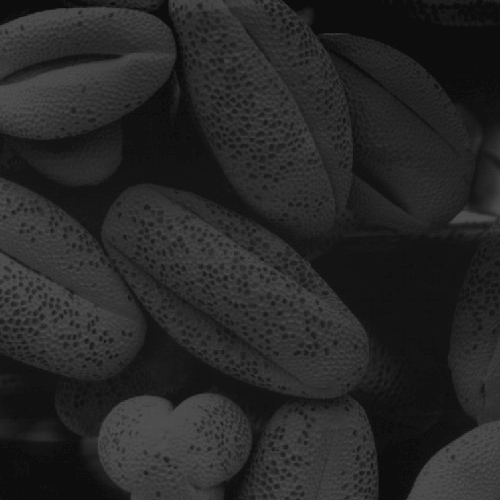
\includegraphics[width=0.3\textwidth]{imgs/Fig3.15(a)1.jpg}}
	\quad
	\subfloat[Imagen 3.15(2)]{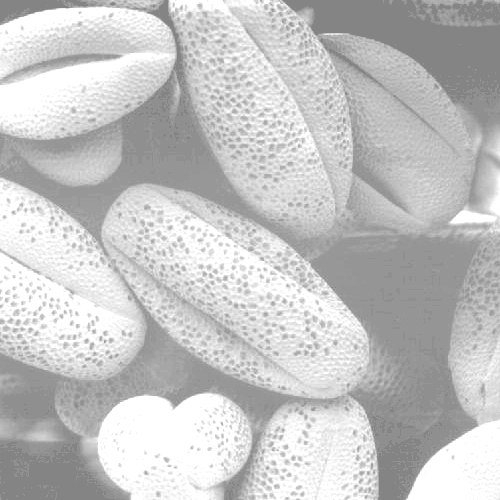
\includegraphics[width=0.3\textwidth]{imgs/Fig3.15(a)2.jpg}}
	\quad
	\subfloat[Imagen 3.15(3)]{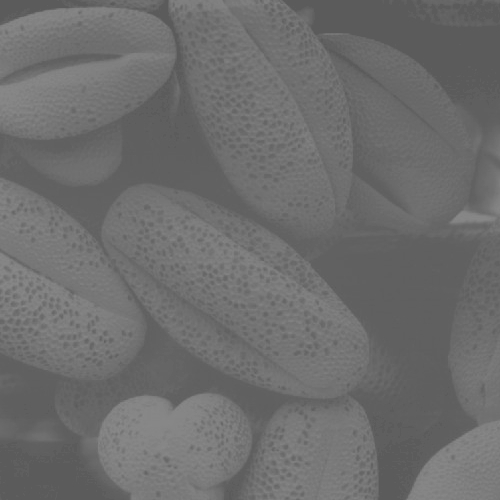
\includegraphics[width=0.3\textwidth]{imgs/Fig3.15(a)3.jpg}}
	\caption{Imágenes utilizadas para evaluar el programa desarrollado.}
	\label{img:test_imgs}
\end{figure}



\subsection{Algoritmos e implementación}

\subsubsection{Histograma de una imagen}

El histograma de una imagen es el conteo del total de píxeles de cierta intensidad presentes en dicha imagen. En nuestro caso, dado que se maneja una escala de grises con 8 bits, la intensidad toma valores entre 0 y 255. 
Además, dado que todas las imágenes de prueba tienen un tamaño de $500\times500$, el total de píxeles será de $250,000$. En las aplicaciones de visión por computadora resulta de más interés el histograma normalizado,
donde se divide el conteo de cada valor de intensidad entre el total de píxeles, de forma que estos valores se restringen en un valor entre 0 y 1. Dado que las imágenes solo toman valores discretos, esto es una aproximación a la \textit{probabilidad} de que cierta intensidad aparezca 
en la imagen.

Para el desarrollo del histograma, se utilizó \textit{opencv} para leer la imagen en escala de grises como una matriz de $500\times500$. Esta matriz se aplanó a un vector de tamaño $1\times25,000$ para simplificar cálculos. Se creó otro vector de ceros con índices de 0 a 255, de tal forma que cada índice se corresponde con cierta intensidad. Este es el utilizado para generar el histograma. Posteriormente, se recorrió el vector de la imagen aplanada, aumentando en 1 el valor del histograma en el índice correspondiente a la intensidad del píxel. Al final de este proceso, se tiene que en el vector histograma el valor correspondiente a cada índice indica el total de píxeles con dicha intensidad en la imagen.

Este programa se implementó como una función de Python que toma como entrada la matriz imagen. Cabe destacar que las paqueterías instaladas incluyen funciones que realizan este proceso, pero se decidió implementarlo desde cero por el valor didáctico. 
\subsubsection{Ecualización de histograma}
Para cada imagen, su histograma correspondiente nos da información acerca de la distribución de tonos. Imágenes oscuras tendrán histogramas centrados a la izquierda del rango de intensidades, imágenes claras tendrán histogramas centrados a la derecha, e imágenes con poco contraste tendrán histogramas ubicados alrededor del centro de este rango. Para la mejora de la calidad de una imagen, buscamos aumentar su rango dinámico, de manera que utilice todas las intensidades disponibles. Esto se traduce en un histograma distribuido de manera uniforme.

Por lo tanto, utilizaremos transformaciones de histogramas para la mejora de la calidad de imágenes. En especifico, se utilizará aquella dada por  
\cite{gonzalezDigitalImageProcessing2017}
$$
s_k = T(r_k) = (L-1) \sum_{j=0}^k p_r(r_j) \quad K = 0, \dots, L-1 
$$
donde $s_k$ indica el valor del píxel resultante, $r_k$ el valor del píxel original, $p_r(r_j)$ la probabilidad de encontrar la intensidad $r_j$ en la imagen, y $L$ es el número total de intensidades posibles. Notemos que, como las imágenes digitales están dadas en valores discretos, la probabilidad de una intensidad dada se puede encontrar con la fórmula
$$
p_r(r_k) = \dfrac{n_k}{\text{Total de pixeles}}
$$
donde $n_k$ indica cuántos píxeles en la imagen tienen la intensidad especificada. Como se mencionó anteriormente, esta información se encuentra de forma explícita en el histograma normalizado. De esta forma, la transformación mostrada se puede aplicar de manera directa teniendo la imagen original y su histograma normalizado.

La función es la \textit{distribución de probabilidad acumulativa discreta.} Resulta de interés dado que, como se demuestra en \cite{gonzalezDigitalImageProcessing2017}
, su equivalente continuo da como resultado una imagen donde las intensidades tienen una probabilidad uniforme, de forma que su histograma es plano, abarcando todo el rango de tonos. Esto no se cumple para el caso discreto, pero sí se logra que el histograma abarque todo el rango de intensidades de tal forma que se mejora el contraste de la imagen en una \textit{gran cantidad de casos}. Como es una transformación global, presenta malos resultados en imágenes donde las tonalidades cambian de forma drástica en diferentes secciones.

Para obtener la probabilidad acumulativa, simplemente debemos realizar una suma acumulativa sobre nuestro histograma normalizado. Aunque esto se encuentra implementado en la paquetería de \textit{numpy}, se implemento desde cero. El resultado de esta suma se escala multiplicándolo por 255, y finalmente se realiza un mapeo sobre la imagen original para obtener la imagen \textit{ecualizada}. Para ello, se utilizan el indexado avanzado de \textit{numpy} sobre esta distribución, guardada como un \textit{array}. Se utiliza como arreglo de índices la imagen original aplanada, de forma que los valores originales de cada píxel llevan a los valores escalados indicados por la distribución acumulativa. Al array resultante se le dan las dimensiones de la imagen original, obteniendo la imagen ecualizada. 

\subsection{Mejora de las imágenes}
Para cada una de las imágenes de prueba se aplicó el siguiente proceso, de acuerdo al script incluido en el anexo:
	\begin{enumerate}
	\item Lectura de la imagen como matriz utilizando \textit{opencv}. A su vez, se crea una copia aplanada de la matriz y se guardan las dimensiones originales.
	
	\item Obtención del histograma de la imagen original utilizando la función desarrollada. Este se normaliza dividiendo entre el total de píxeles de la imagen.
	
	\item Calculo de la distribución de probabilidad acumulada mediante una suma acumulativa sobre el histograma normalizado. Esta se escala multiplicando por el rango dinámico, 255.
	
	\item Creación de la nueva imagen ecualizada mediante la probabilidad acumulada escalada. Esta se crea primero como una matriz aplanada, y después se le dan las dimensiones de la imagen original.
	
	\item Se grafica la imagen original junto a su histograma con la función desarrollada para ello. Se hace lo mismo con la imagen ecualizada.
	
	\item Se grafica la función de ecualización, esto es, la distribución de probabilidad escalada. 
	\end{enumerate}

Todas las operaciones de matrices se realizaron con \textit{numpy}, y las gráficas se obtuvieron mediante \textit{matplotlib}. Se utilizaron de consulta las fuentes \cite{SolemsVisionBlog2015}, \cite{karnewarBacktobasicsPart12018} y \cite{walkerHistogramEqualizationPython2023}.

\section{Resultados}
Se muestran las imágenes originales, los resultados de la ecualización, los histogramas correspondientes a cada imagen y su función de distribución escalada en las figuras \ref{img:resultados 1}, \ref{img:resultados 2}, \ref{img:resultados 3}.  

 \begin{figure}[htbp]
	\centering
	\subfloat[Imagen original y su histograma]{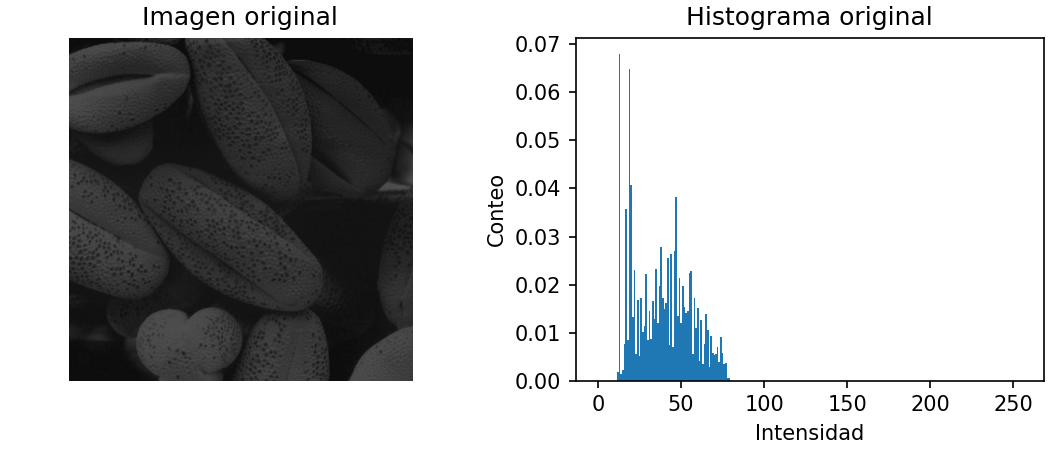
\includegraphics[width=0.9\textwidth]{imgs/original1.png}}
	\quad
	\subfloat[Imagen ecualizada y su histograma]{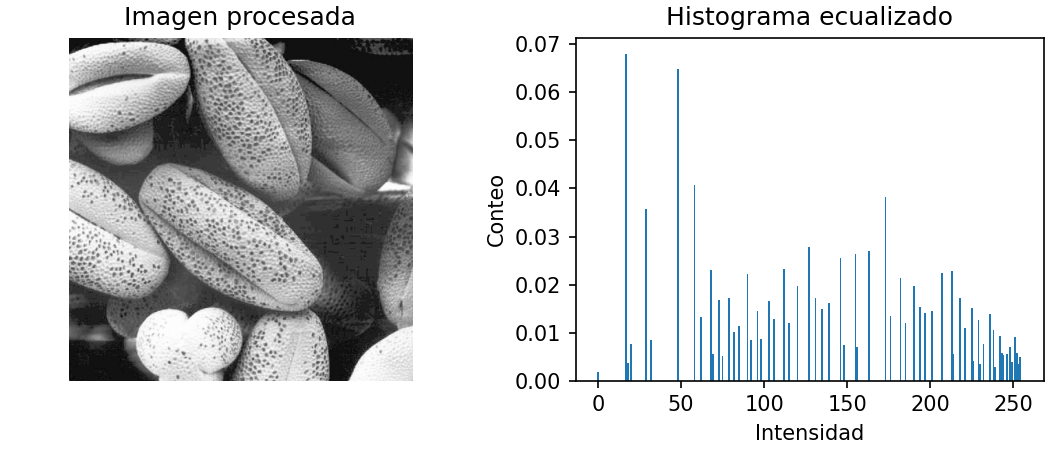
\includegraphics[width=0.9\textwidth]{imgs/resultado1.png}}
	\quad
	\subfloat[Función de transformación del histograma]{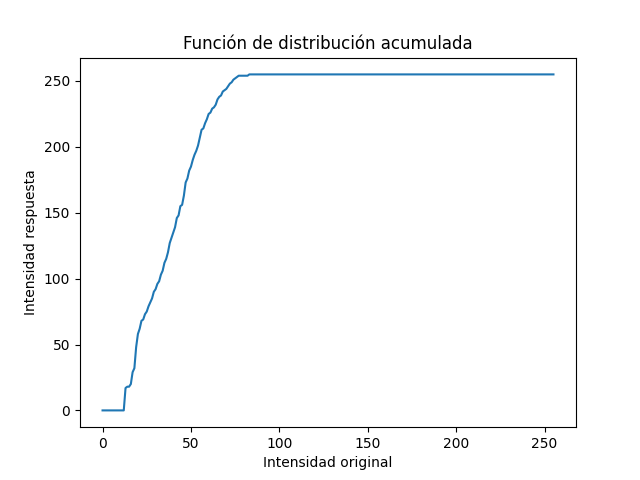
\includegraphics[width=0.5\textwidth]{imgs/cdf1.png}}
	\caption{Resultados para la imagen 3.15(1).}
	\label{img:resultados 1}
\end{figure}

\begin{figure}[htbp]
	\centering
	\subfloat[Imagen original y su histograma]{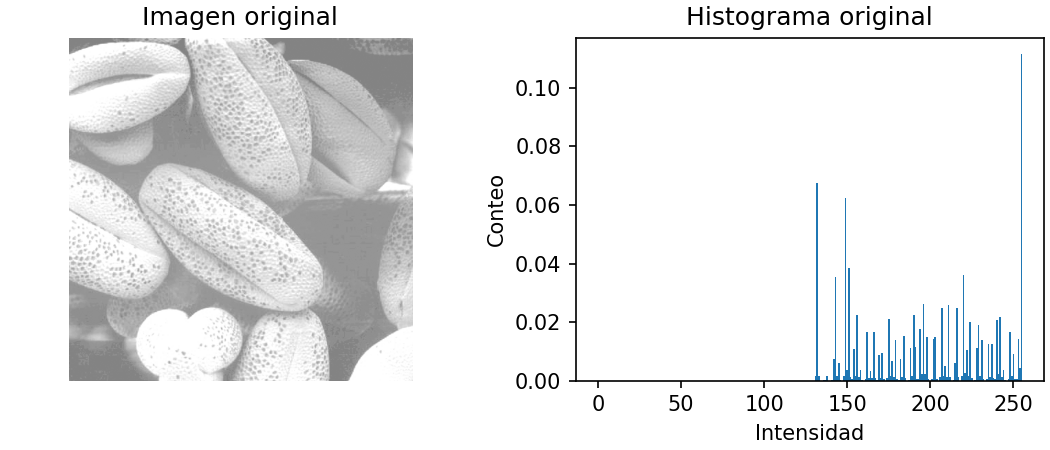
\includegraphics[width=0.9\textwidth]{imgs/original2.png}}
	\quad
	\subfloat[Imagen ecualizada y su histograma]{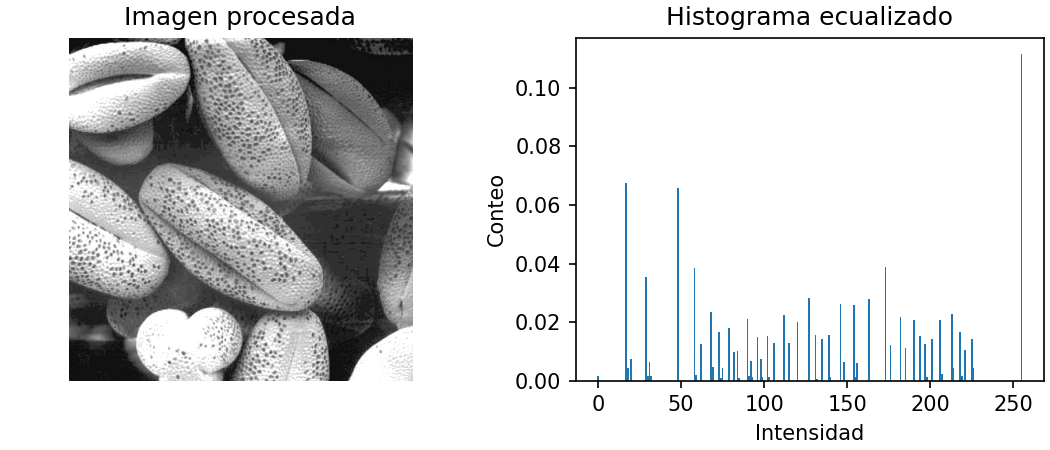
\includegraphics[width=0.9\textwidth]{imgs/resultado2.png}}
	\quad
	\subfloat[Función de transformación del histograma]{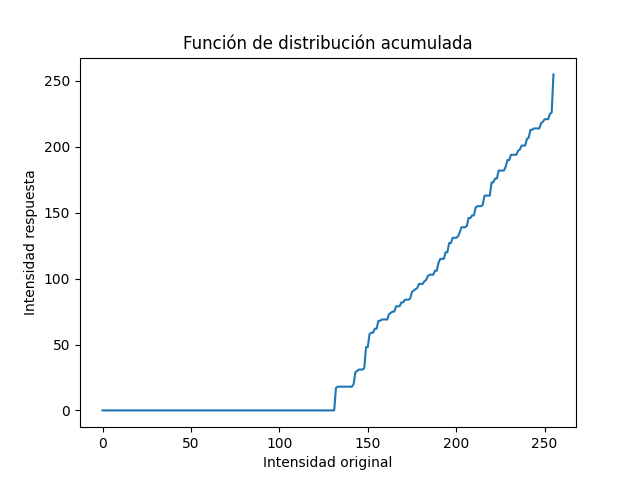
\includegraphics[width=0.5\textwidth]{imgs/cdf2.png}}
	\caption{Resultados para la imagen 3.15(2).}
	\label{img:resultados 2}
\end{figure}

\begin{figure}[htbp]
	\centering
	\subfloat[Imagen original y su histograma]{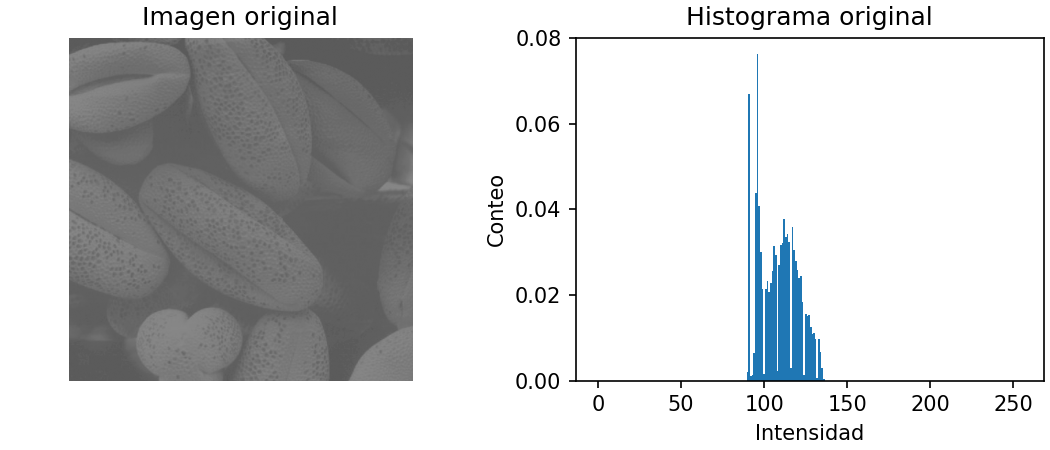
\includegraphics[width=0.9\textwidth]{imgs/original3.png}}
	\quad
	\subfloat[Imagen ecualizada y su histograma]{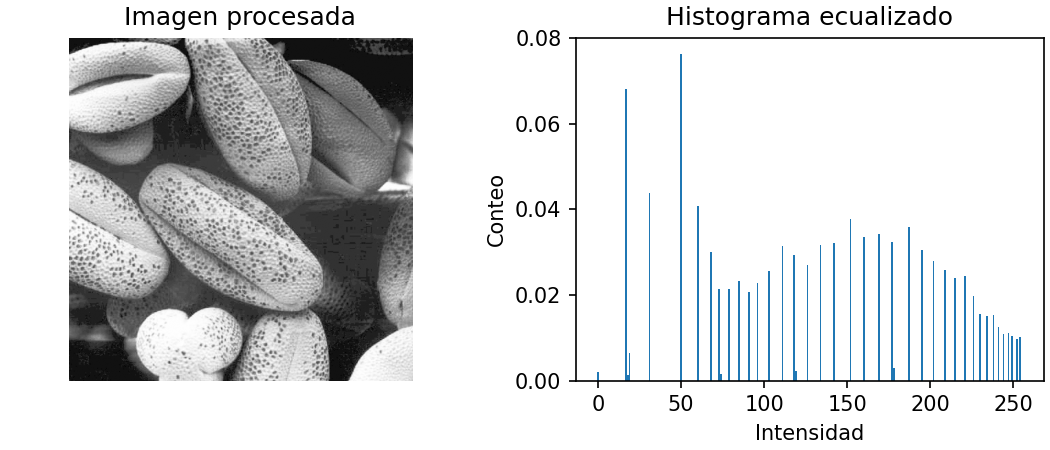
\includegraphics[width=0.9\textwidth]{imgs/resultado3.png}}
	\quad
	\subfloat[Función de transformación del histograma]{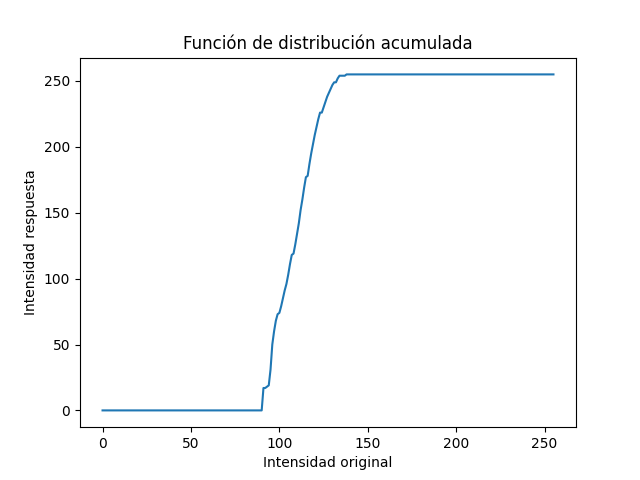
\includegraphics[width=0.5\textwidth]{imgs/cdf3.png}}
	\caption{Resultados para la imagen 3.15(3).}
	\label{img:resultados 3}
\end{figure}

A pesar de tener histogramas diferentes, las tres imágenes resultantes son extremadamente similares, sin diferencias perceptibles a simple vista. Esto es de esperarse, dado que todas toman como base la misma imagen, con diferentes contrastes. Al eliminar las deficiencias causadas por estos contrastes extremos, obtenemos la imagen base. Todos los histogramas resultantes comparten el que se abarca todo el rango dinámico, desde el 0 hasta el 255, y el que una gran cantidad de los valores intermedios se encuentran vacíos. Esto es evidente al observar las funciones de transformación, donde todas presentas zonas planas que envían todo un rango de valores a la misma respuesta. 

\section{Conclusiones}
Para las imágenes de prueba seleccionadas, la ecualización de histograma tuvo resultados excepcionales, permitiendo una gran mejora de los detalles observables en la imagen, aumentando el rango dinámico y en general mejorando la calidad de imagen. Sin embargo, esto funciona dado que todas presentan un tono similar de manera global: toda la imagen 3.15(1) es oscura, toda la imagen 3.15(2) es clara, y toda la imagen 3.15(3) presenta un tono apagado. Si estas tuvieran regiones muy marcadas dentro de la misma imagen, esto es, una zona oscura contrastada con una zona muy clara, el filtro sería incapaz de manejarlo de manera adecuada. Esto se puede resolver aplicando la ecualización por zonas sobre la imagen, o utilizando otros métodos de histograma más sofisticados. Aunque en este trabajo se limitó su uso a imágenes en escala de gris, la expansión a imágenes RGB se da de manera natural, aplicando el mismo proceso a cada uno de los canales de color. 


\bibliographystyle{plain}
\bibliography{histograma_fuentes.bib}

\newpage

\section{Anexo}
\subsection{Lista de paqueterías y versiones}
\begin{itemize}
	\item contourpy==1.3.1
	\item cycler==0.12.1
	\item fonttools==4.56.0
	\item kiwisolver==1.4.8
	\item matplotlib==3.10.0
	\item numpy==2.2.3
	\item opencv-python==4.11.0.86
	\item packaging==24.2
	\item pillow==11.1.0
	\item pyparsing==3.2.1
	\item python-dateutil==2.9.0.post0
	\item six==1.17.0
\end{itemize}

\subsection{Código}

\lstinputlisting[language=python]{/home/ulisex/Documentos/Maestria IA/Semestre 2/Vision por computadora/Tarea3_histograma/hist_eql.py}

\end{document}